\chapter{Opis projektnog zadatka}
		
		{Zdravlje i fizička aktivnost prioritet su svakoj osobi. U današnje vrijeme kada većina živi užurbanim, zaposlenim životima, teško je u vlastiti raspored uključiti i  tjelovježbu. Svakodnevne obaveze razlikuju se iz dana u dan te se ponekad čini nemogućim pohađati striktno određene termine treninga. Rješenje je tih problema web aplikacija "Group Fitness Planner".}
		
		{Cilj je ovoga projekta razviti programsku podršku za navedenu aplikaciju. Ona će korisniku omogućiti da vrijeme treninga prilagođava svom slobodnom vremenu u skladu s osobnim planom vježbanja.}
		
		{Prilikom pokretanja aplikacije prikazuje se naslovnica web aplikacije. Na njoj, prikazane su informacije o aplikaciji, u gornjem lijevom kutu nalazi se logo aplikacije, a u gornjem desnom kutu nalazi se poveznica za prijavu korisnika. Klikom na poveznicu, prikazuje se okvir u koji se upisuju podaci za prijavu korisnika, to jest korisničko ime i lozinka. U slučaju da korisnik nema račun, na dnu okvira također se nalazi poveznica koja vodi do stranice za registraciju korisnika. Za kreiranje novoga računa potrebni su idući podaci:}
		\begin{packed_item}
			\item {ime}
			\item {prezime}
			\item {korisničko ime}
			\item {e-mail adresa}
			\item {lozinka}
			\item {cilj korisnika}
		\end{packed_item}
		
		{Registracijom u sustav korisniku se dodjeljuju prava klijenta. Registrirani korisnik može pregledati osobne podatke, mijenjati ih te izbrisati korisnički račun.}
		
		{\textit{Korisnik treninga} prilikom registracije odabire ciljeve koje želi postići vježbanjem. Sukladno odabranim ciljevima, korisniku se dodjeljuju vrste treninga koji dovode do ostvarenja tih ciljeva. Registracijom ili prijavom,  korisniku se prikazuje kalendar tekućeg mjeseca i poruka „Molimo Vas pričekajte da Vam trener dodijeli vježbe.“ Nakon što su vježbe dodijeljene, korisniku su prikazani datumi u kalendaru u kojima se odvijaju treninzi koji sadržavaju te vježbe. Odabirom određenog termina, prikazuje se naziv treninga s opisanim vježbama koje su uključene u trening i imenom trenera. Korisnik odabire vrijeme koje mu odgovara te klikom na gumb rezervira trening. Odabrani cilj moguće je mijenjati početkom svakoga mjeseca. Ako korisnik želi na početku novog mjeseca promijeniti cilj odlazi na stranicu s informacijama o svom korisničkom profilu. Na toj stranici nalaze se opći podaci o korisniku kao što su ime, prezime, korisničko ime, email adresa, fond preostalih sati i odabrani ciljevi. Tamo korisnik može promijeniti jedan ili više ciljeva ili nadodati nove ciljeve. Promjenom ciljeva, mijenjaju s i preporučene vježbe, a time i izbor treninga.}
		
		{\textit {Trener} ima pristup profilima registriranih korisnika te u skladu s ciljevima koje je korisnik odabrao dodjeljuje korisniku vježbe. Prijavom u aplikaciju prikazuje mu se popis imena i ciljeva svih registriranih korisnika. Pored imena onih korisnika koji nemaju dodijeljene vrste vježbi, prikazuje mu se gumb "Dodijeli vježbe". Također, trener na početku svakog mjeseca, u aplikaciju postavlja nove termine treninga te maksimalan kapacitet korisnika određenog termina. Osim toga, treneri za svaki trening odlučuju koje su vrste vježbi sadržane u treningu te se prema tome korisnicima dodjeljuju termini treninga koji sadrže vježbe preporučene za njih. Dodatno, treneri određuju pravila po kojima korisnici smiju rezervirati treninge. Ta su pravila da korisnik može rezervirati maksimalno pet treninga tjedno, smije rezervirati samo jedan trening tjedno intenzivnog karaktera te maksimalno dva treninga dnevno.}
		
		{\textit {Administrator} sustava ima najviše ovlasti. On ima pristup bazi podataka s popisom registriranih korisnika i njihovim podacima. Također, administrator trenerima dodjeljuje njihov status. Uz to, ažurira sve podatke u aplikaciji. }
		
		
		{Web aplikacije slične našoj već postoje na tržištu. Neke od njih su web aplikacija za rezervaciju treninga u teretani \textit{"Adidas Sports Studio"} (prikaz na slici \ref {fig:adidassportsstudio1} i \ref{fig:adidassportsstudio2}) i web aplikacija za teretanu \textit{"Sparta Gym"} (slika \ref{fig:spartagym1}). Ono što našu aplikaciju razlikuje od već prisutnih, personalizirani je pristup korisniku. Na navedenim aplikacijama, svim korisnicima prikazuje se cjelokupni raspored treninga koji se odvijaju u navedenim teretanama. S druge strane, u našoj aplikaciji ovisno o cilju korisnika, trener dodjeljuje vježbe te se prema tim vježbama prikazuju određeni termini treninga. To dodatno motivira korisnike treninga jer znaju kako su baš ti trenizi namijenjeni njima te će ih dovesti do željenih rezultata. Također, korisnici prije dolaze do napretka, a to ih dodatno motivira za nastavak.} 
		
		
		\begin{figure}[H]
			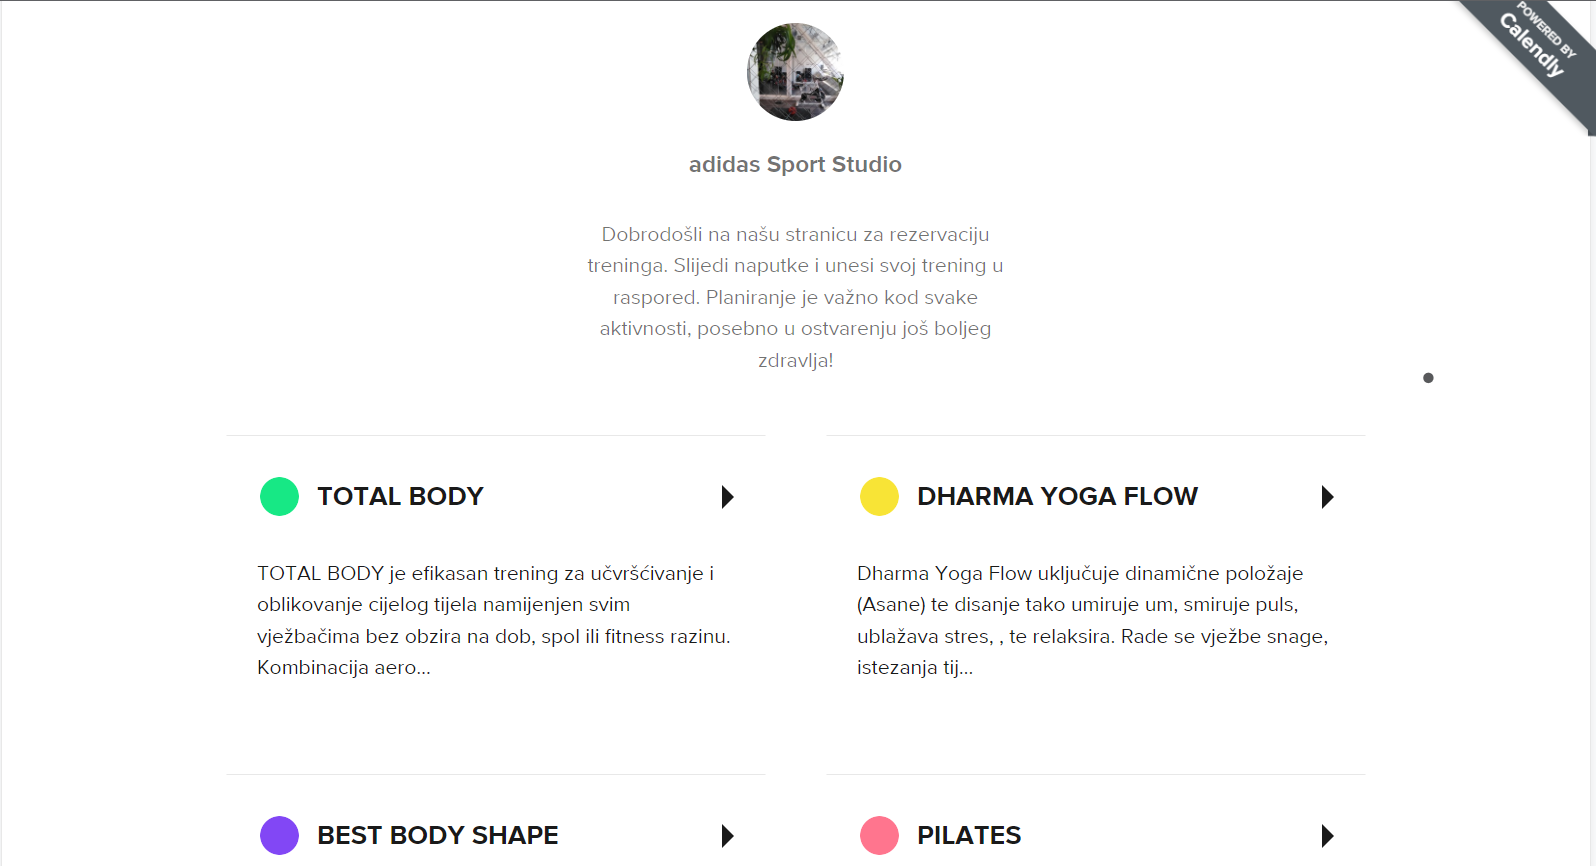
\includegraphics[scale=0.3]{slike/adidassportsstudio1.PNG} %veličina slike u odnosu na originalnu datoteku i pozicija slike
			\centering
			\caption{"Adidas Sports Studio" web aplikacija}
			\label{fig:adidassportsstudio1}
		\end{figure}
		
		\begin{figure}[H]
			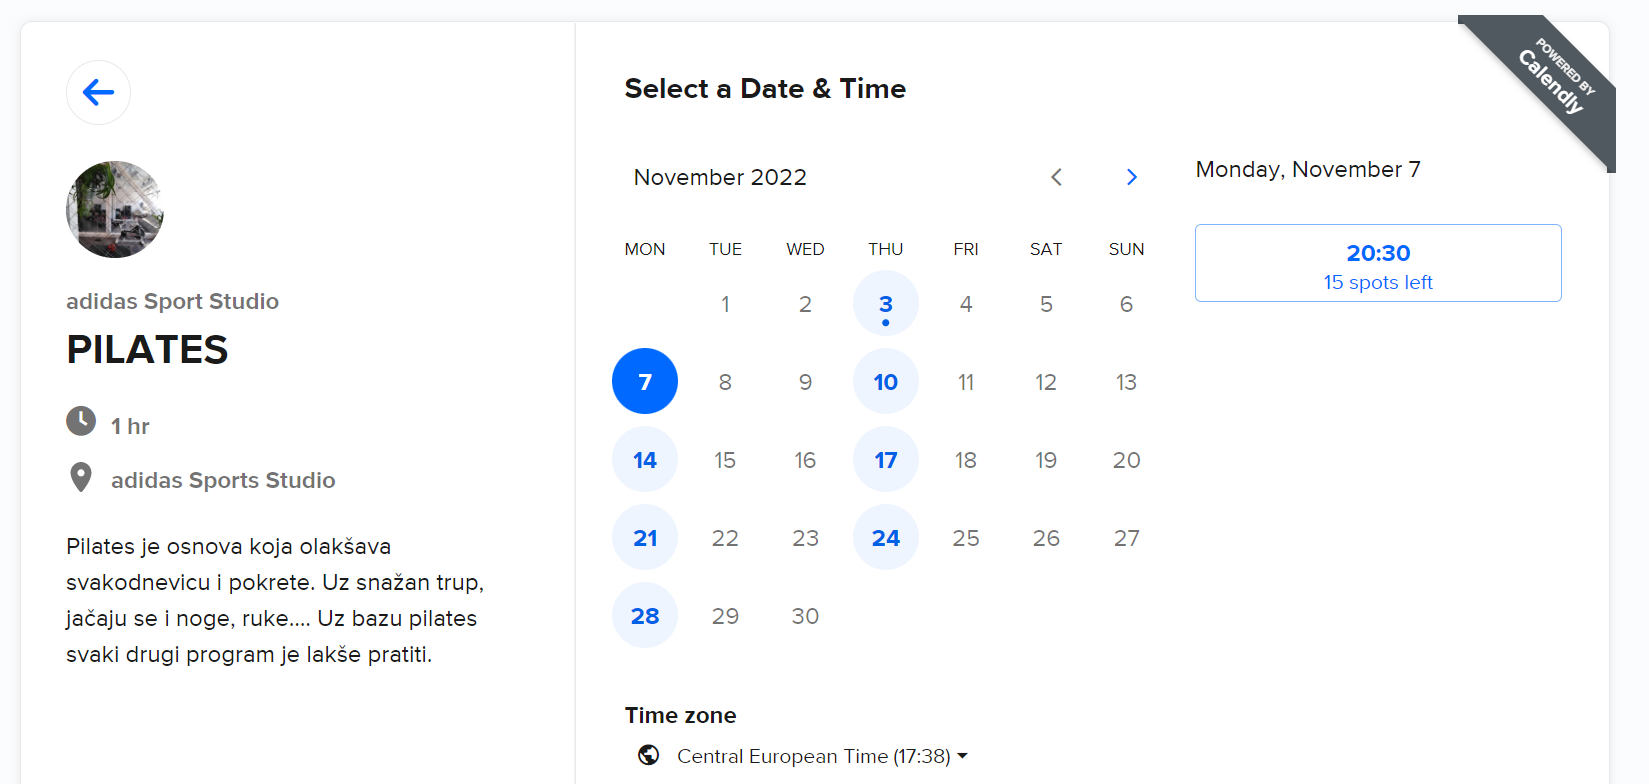
\includegraphics[scale=0.3]{slike/adidassportsstudio2.PNG} %veličina slike u odnosu na originalnu datoteku i pozicija slike
			\centering
			\caption{"Adidas Sports Studio" web aplikacija}
			\label{fig:adidassportsstudio2}
		\end{figure}
		
		\begin{figure}[H]
			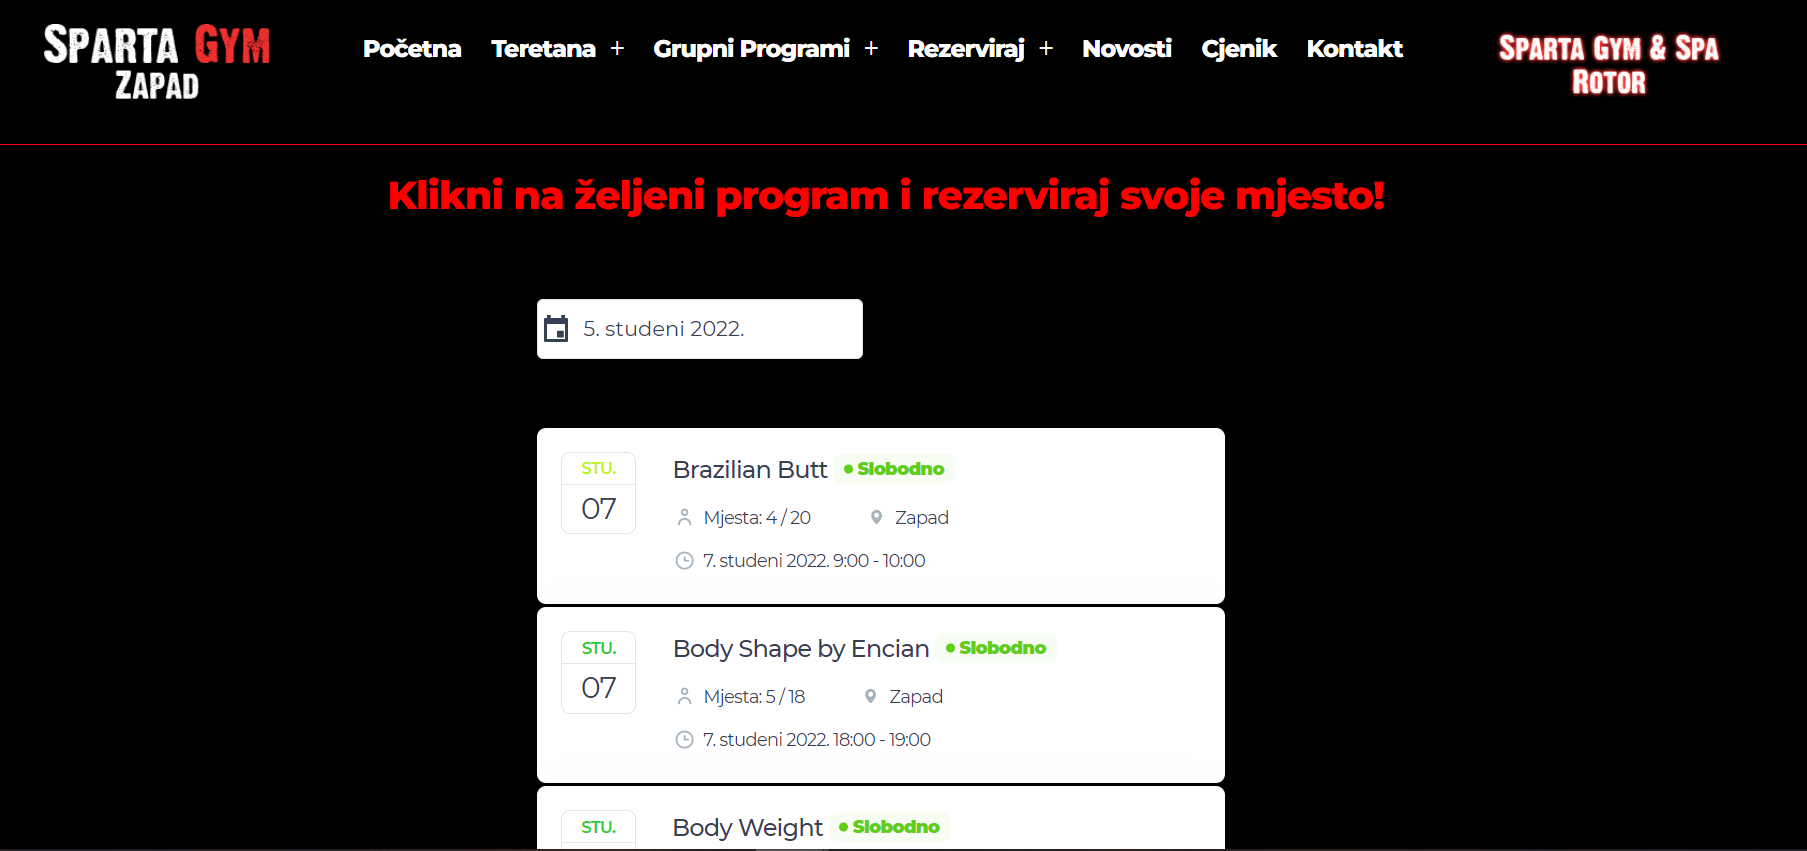
\includegraphics[scale=0.3]{slike/spartagym1.PNG} %veličina slike u odnosu na originalnu datoteku i pozicija slike
			\centering
			\caption{"Sparta Gym" web aplikacija}
			\label{fig:spartagym1}
		\end{figure}
		
		{Upravo zbog tog personaliziranog pristupa, smatramo da će aplikacija biti korisna svima onima koji nemaju vremena istražiti i inforimirati se o tome koje vrste vježbi bi najviše odgovarale njihovim potrebama.} 
		
		{Također, postoji puno prostora za nadogradnju aplikacije. jedan primjer je povezivanje nekoliko sportskih objekata u aplikaciji. Veliki broj tvrtki svojim zaposlenicima nudi korištenje "Multisport" kartice. To je kartica kojom je omogućen pristup velikom broju sportskih objekata u cijeloj Hrvatskoj. Tako bi aplikacija mogla nuditi termine treninga u različitim teretanama i sportskim prostorima. Time bi korisnici koji često putuju mogli rezervirati termine i u drugim gradovima te tako biti još redovitiji u pohađanju treninga. Drugi je primjer proširenja aplikacije da se uz tenere, uključe i stručnjaci na nekim drugim područjima osim fitnessa. Jedan primjer su nutricionisti. Ovisno o ciljevima koje korisnik odabire, nutricionist mu preporuča prehrambene namirnice koje bi bilo poželjno da uvrsti u vlastitu prehranu. Korisniku bi se tako uz termine treninga u kalendaru prikazivao i  jelovnik koji uključuje obroke koji sadrže preporučene namirnice. }
		
		
		\eject
		
	